\documentclass[11pt, oneside]{article} 
\usepackage{geometry}
\geometry{letterpaper} 
\usepackage{graphicx}
	
\usepackage{amssymb}
\usepackage{amsmath}
\usepackage{parskip}
\usepackage{color}
\usepackage{hyperref}

\graphicspath{{/Users/telliott/Github/precalculus/fig/}}
% \begin{center} 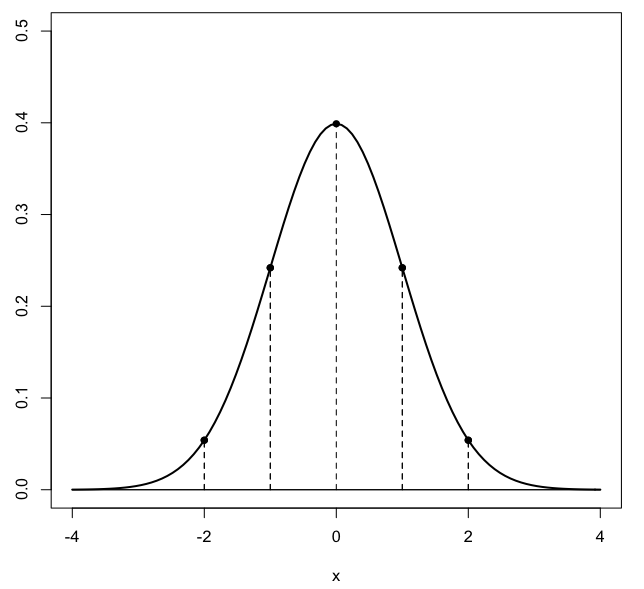
\includegraphics [scale=0.4] {gauss3.png} \end{center}

\title{Irrational numbers}
\date{}

\begin{document}
\maketitle
\Large

\subsection*{continued fractions}
Square roots can be represented as continued fractions.  Some smart person figured out that we can write this:
\[ (\sqrt{2} - 1)(\sqrt{2} + 1) = 2 - 1 = 1 \]

Now, rearrange to get a substitution we will use repeatedly
\[ \sqrt{2} - 1 = \frac{1}{\sqrt{2} + 1} \]

Add one and subtract one on the bottom right:
\[ \sqrt{2} - 1 =  \frac{1}{2 + \sqrt{2} - 1} \]

And substitute for $\sqrt{2} - 1$:
\[ = \frac{1}{2 + \frac{1}{\sqrt{2} + 1}} \]

Lather, rinse, and repeat:
\[ = \frac{1}{2 + \frac{1}{2 + \sqrt{2} - 1}} = \frac{1}{2 + \frac{1}{2 + \frac{1}{\sqrt{2} + 1} }} \]

Clearly, this goes on forever.
\[ \sqrt{2} - 1 =  \cfrac{1}{2+\cfrac{1}{2+\cfrac{1}{2 + \dots}}}  \]

Add $1$ to the value of the \emph{continued fraction} to get an expression for the square root of $2$.

The numerators are all $1$, so this is called a simple continued fraction.  The continued fraction representation of $\sqrt{2}$ is usually written as $[1:2]$, meaning that there is an initial $1$ followed by repeated $2$'s.

This fraction goes on forever (since $\sqrt{2}$ is irrational).  One can view the existence of the infinite continued fraction as a proof of irrationality.

We can turn the above into an approximate decimal representation of $\sqrt{2}$, by truncating the infinite expansion at the $\dots$.  Then the last fraction is $5/2$.  Invert and add, repeatedly:

\begin{verbatim}
2 + 1/2 = 5/2
2 + 2/5 = 12/5
2 + 5/12 = 29/12
2 + 12/29 = 70/29
2 + 29/70 = 169/70
2 + 70/169 = 408/169
\end{verbatim}

To terminate we need to use that initial $1$:
\begin{verbatim}
1 + 169/408 = 577/408 = 1.414216
\end{verbatim}

To six places, $\sqrt{2} = 1.414213$.  We have five places, and can easily get more.

\subsection*{approximations}

In all cases we write particular real numbers as \emph{approximations}.  For example, the square root of $2$ lies between $1$ and $2$ because
\[ 1^2 = 1 < 2 \]
\[ 2^2 = 4 > 2 \]

Implying that $\sqrt{2} < 2$.  At the second place:
\[ 1.4^2 = 1.96 < 2 \] 
\[1.5^2 = 2.25 > 2 \]

Implying that $\sqrt{2} < 1.5$.  At the third:
\[ 1.41^2 = 1.9881 < 2 \]
\[1.42^2 = 2.0164 > 2 \]

Implying that $\sqrt{2} < 1.42$.  

This process may be continued for as long as desired. 

We can never write down the decimal value of $\sqrt{2}$ exactly, but only approximate it to greater and greater precision.  It goes on forever.

In carrying out this recursive process, suppose we know $1.41$ and we seek the next digit.  Rather than try all the digits in order starting with $1$, there is a better way.

Try to estimate the error from the previous round.  

For example $1.41^2 = 1.9881$ so we are short of $2.0000$ by $0.0119$.  

$1.42^2 = 2.0164$ so the difference is $0.0283$ and the fraction of the difference that we're under is $119/283 = 0.4205$.  In fact, the next two digits of the approximation to $\sqrt{2}$ are $42$.

However, we will see a much better method for obtaining this value later, called Newton's method.

At the seventh place
\[ 1.414213^2 = 1.9999984093689998.. < 2 \]
\[ 1.414214^2 = 2.0000012377960004 > 2 \]

Because any repeating decimal can be written as a fraction, we know that the sequence cannot repeat (any apparent repeat will be illusory).  

It is a curious fact that all the digits of $\pi$, \emph{to whatever accuracy you desire}, can be found in the correct order, somewhere within the digital expansion of $e$ or $\phi$ or indeed, any irrational number.  The converse is also true.

Another way to say the same thing is that \emph{any} finite sequence can be found within \emph{any} infinite sequence, and in as many copies as you have the patience to discover.  The sequence 271828 is found starting around digit 33,790 of $\pi$, but 2718281 (adding the next digit of $e$) is not found within the first million digits of $\pi$.  You just need more.

\subsection*{limit of a sequence}

The real number $\sqrt{2}$ is defined to be the limit of the sequence 

$1.4, 1.41, 1.414, \dots 1.414214 \dots$ 

as the number of terms $n \rightarrow \infty$.

In a similar way, the number $e$ can be viewed as
\[ \lim_{n \rightarrow \infty} (1 + \frac{1}{n})^n \]

And the number $\pi$ can be viewed as the limit of the method of exhaustion applied to the area of a unit circle.

\end{document}